\appendix

\section{Tagging procedure}
\label{Taggingprocedure}

\setcounter{table}{0} \renewcommand{\thetable}{A.\arabic{table}}
\setcounter{figure}{0} \renewcommand{\thefigure}{A.\arabic{figure}}

The following description is adapted from \citet{Verhelst2018}. 100 Eels were caught and tagged at the tidal weir in Merelbeke in the Zeeschelde during late summer and autumn (September–November) of three consecutive years (2015 till 2017) using double fyke nets. After periods of heavy rain, water flows over the sluices allowing eels to swim over the sluices. Placing the fyke nets behind the sluices and during periods of heavy rain, allowed to coordinate capture events and improve the chance of capturing eel. Several morphometric features were measured in order to determine the eel maturation stage \citep{Durif2005}: Total length (TL, to the nearest mm), body weight (W, to the nearest g), the vertical and horizontal eye diameter (EDv and EDh respectively, to the nearest 0.01 mm) and the length of the pectoral fin (FL, to the nearest 0.01 mm) (Table \ref{dimensionsTaggedEels}). Only females were tagged, since males are smaller than the minimum size handled in this study (< 450 mm \citep{Durif2005}). Eels of three different maturation stages were tagged: premigrant (F3, n = 51) and the two migrant stages F4 and F5 (n = 21 and n = 28, respectively). The eels were tagged with V13 coded acoustic transmitters (13 x 36 mm, weight in air 11 g, frequency 69 kHz, ping frequency: 60–100 s; estimated battery life: 1021-1219 days (battery life time depended on specific transmitter settings), (Table \ref{settingsTaggedEels})) from VEMCO Ltd (Canada). After anesthetizing them with 0.3 ml/L clove oil, tags were implanted with permanent monofilament \citep{Thorstad2013b}. Eels recovered in a quarantine reservoir for approximately one hour and were subsequently released at the nearest receiver. 

Four flounders were tagged with external V7 tags and released at the weir in Mechelen of the Dijle river, a tributary of the Scheldt estuary via the Rupel. A needle with nylon tread was used to attach the tag to the skin, just above the anal fin. The tag was attached on the dorsal side of the fish. Two rubber plates were attached on both sides of the fish to prevent rupture of the skin. On the dorsal side the rubber plate was attached between the skin and the tag. The tags were set to have a low power output and a ping frequency of 40 to 80 seconds.

\begin{table}[]
\centering
\scriptsize
\caption{Number of all tagged female eels per stage with the different morphometrics: total length (TL), body weight (BW), horizontal and vertical eye diameters (EDh and EDv, respectively) and pectoral fin length (FL). Mean, standard deviation and range (between brackets) are indicated (Adopted from \citet{Verhelst2018}).}
\label{dimensionsTaggedEels}
\begin{tabular}{|l|l|l|l|l|l|l|}
\hline
Stage & Number & TL (mm)                                                         & BW (g)                                                             & EDh (mm)                                                               & EDv (mm)                                                              & FL (mm)                                                                 \\ \hline
F3  & 51     & \begin{tabular}[c]{@{}l@{}}$702 \pm $57 \\ (568 - 835)\end{tabular} & \begin{tabular}[c]{@{}l@{}}$674 \pm $165 \\ (324 - 1106)\end{tabular}  & \begin{tabular}[c]{@{}l@{}}$8.08 \pm $0.57 \\ (6.77 - 9.08)\end{tabular}   & \begin{tabular}[c]{@{}l@{}}$7.55 \pm $0.60 \\ (6.20 - 9.70)\end{tabular}  & \begin{tabular}[c]{@{}l@{}}$32.92 \pm $3.29 \\ (26.76 - 40.32)\end{tabular} \\ \hline
F4   & 21     & \begin{tabular}[c]{@{}l@{}}$810 \pm $57 \\ (707 - 932)\end{tabular} & \begin{tabular}[c]{@{}l@{}}$1162 \pm $217 \\ (771 - 1830)\end{tabular} & \begin{tabular}[c]{@{}l@{}}$10.41 \pm $0.92 \\ (9.13 - 12.49)\end{tabular} & \begin{tabular}[c]{@{}l@{}}$9.66 \pm $0.78 \\ (8.60 - 11.86)\end{tabular} & \begin{tabular}[c]{@{}l@{}}$40.86 \pm $4.32 \\ (30.84 - 48.18)\end{tabular} \\ \hline
F5    & 28     & \begin{tabular}[c]{@{}l@{}}$662 \pm $56 \\ (575 - 775)\end{tabular} & \begin{tabular}[c]{@{}l@{}}$585 \pm $144 \\ (417 - 912)\end{tabular}   & \begin{tabular}[c]{@{}l@{}}$9.33 \pm $0.80 \\ (8.14 - 11.18)\end{tabular}  & \begin{tabular}[c]{@{}l@{}}$8.80 \pm $0.79 \\ (7.62 - 10.39)\end{tabular} & \begin{tabular}[c]{@{}l@{}}$34.41 \pm $3.68 \\ (28.97 - 45.37)\end{tabular} \\ \hline
\end{tabular}
\end{table}

\begin{table}[]
\centering
\scriptsize
\caption{The number and settings of the transmitters of all tagged eels per step: power output (PO; L = low power output, H = high power output), ping frequency (s) and the time duration (days) per step as well as the total battery life time (days). (Adopted from \citet{Verhelst2018})}
\label{settingsTaggedEels}
\begin{tabular}{|l|l|l|l|l|l|l|l|}
\hline
\multirow{2}{*}{\begin{tabular}[c]{@{}l@{}}Number \\ of \\ transmitters\end{tabular}} & \multicolumn{3}{l|}{Step 1}                                                                                                        & \multicolumn{3}{l|}{Step 2}                                                                                                        & \multirow{2}{*}{\begin{tabular}[c]{@{}l@{}}Battery \\ life \\ (days)\end{tabular}} \\ \cline{2-7}
                                                                                      & PO & \begin{tabular}[c]{@{}l@{}}Ping \\ frequency \\ (s)\end{tabular} & \begin{tabular}[c]{@{}l@{}}Duration \\ (days)\end{tabular} & PO & \begin{tabular}[c]{@{}l@{}}Ping \\ frequency \\ (s)\end{tabular} & \begin{tabular}[c]{@{}l@{}}Duration \\ (days)\end{tabular} &                                                                                    \\ \hline
20                                                                                    & L  & 60 - 100                                                         & 1216                                                       & NA & NA                                                               & NA                                                         & 1216                                                                               \\ \hline
40                                                                                    & H  & 60 - 100                                                         & 120                                                        & L  & 60 - 100                                                         & 901                                                        & 1021                                                                               \\ \hline
40                                                                                    & H  & 60 - 100                                                         & 120                                                        & L  & 60 - 100                                                         & 902                                                        & 1022                                                                               \\ \hline
\end{tabular}
\end{table}

\begin{table}[]
\centering
\scriptsize
\caption{Total length (TL) and body weight (BW) of the tagged flounders}
\label{dimensionsTaggedFlounder}
\begin{tabular}{|l|l|l|}
\hline
Transmitter    & TL (mm) & BW (g) \\ \hline
A69-1601-34454 & 261     & 282    \\ \hline
A69-1601-34455 & 298     & 272    \\ \hline
A69-1601-34456 & 315     & 376    \\ \hline
A69-1601-34460 & 339     & 496    \\ \hline
\end{tabular}
\end{table}

\begin{figure}[h!]
  \centering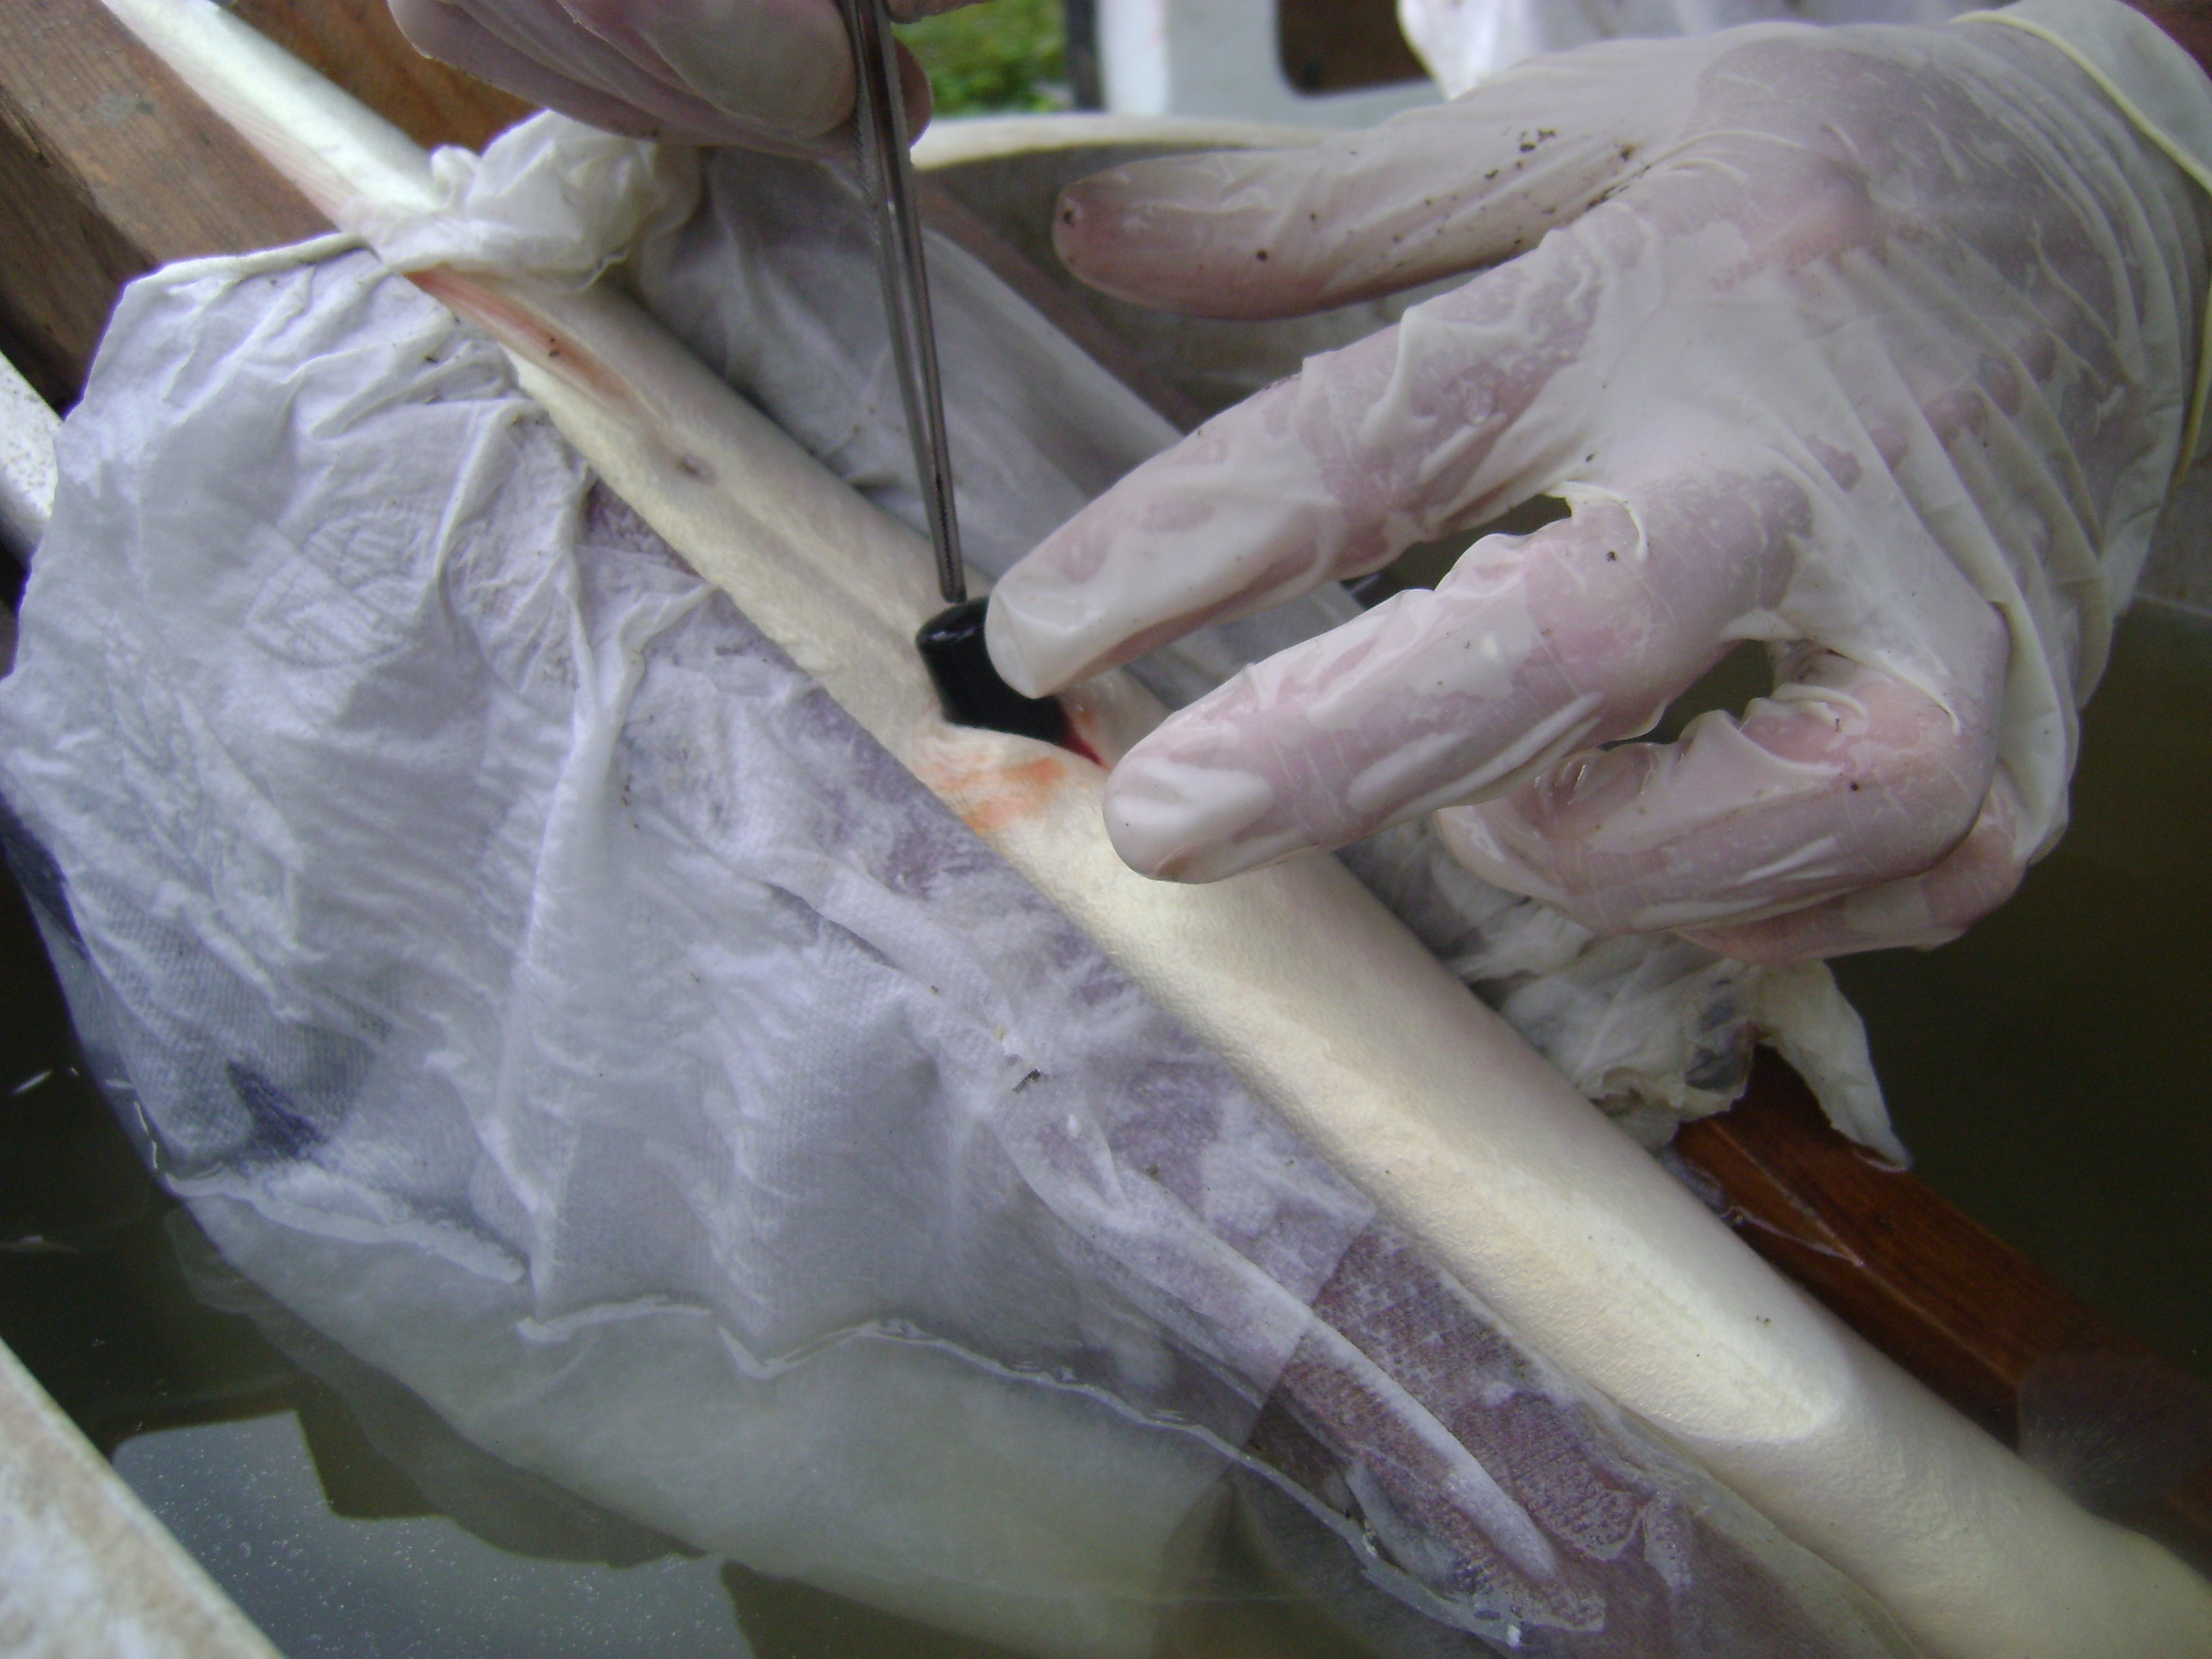
\includegraphics[scale=0.37]{Eeltagged}
  \caption{Internal tagging of eel (\textit{Anguilla anguilla}) with a V13 tag (picture provided by Verhelst P.).}
  \label{fig:Eeltagged}
\end{figure}

\begin{figure}[h!]
  \centering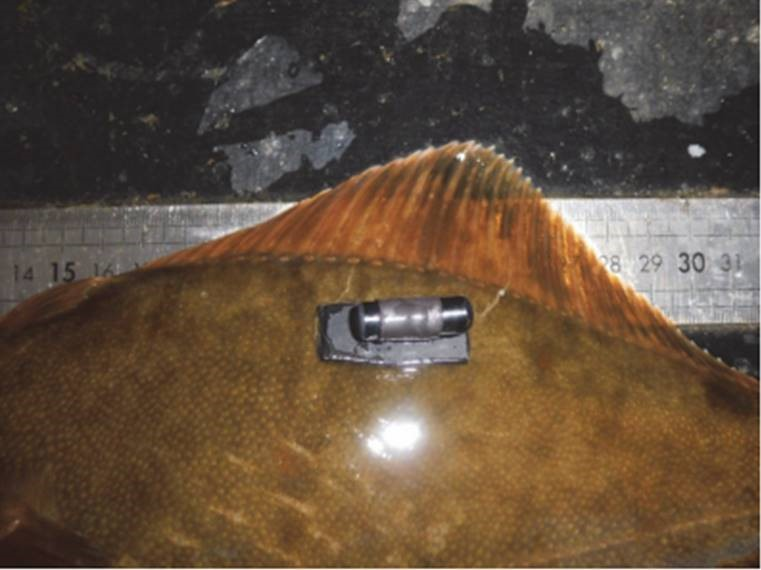
\includegraphics[scale=0.57]{Floundertagged}
  \caption{External tagging of flounder (\textit{Platichthys flesus}) with a V7 tag (picture provided by Verhelst P.).}
  \label{fig:Floundertagged}
\end{figure}

\clearpage

\section{Data processing}
\label{Dataprocessing}
\FloatBarrier

\setcounter{table}{0} \renewcommand{\thetable}{B.\arabic{table}}
\setcounter{figure}{0} \renewcommand{\thefigure}{B.\arabic{figure}}

This practical example describes how detection groups are transformed in residencies-between receivers: Consider a network of three gates \RNum{1}, \RNum{2} and \RNum{3}, spatially aligned as such (Fig. \ref{fig:detectionInterval}). A tagged fish has a detection group \RNum{1}-\RNum{2} with a time lapse of 0.5 hour (type 1A) and another detection group \RNum{1}-\RNum{3} with a time lapse of 1 hour (type 2), which is probably because the fish swam from \RNum{1} to \RNum{2} in 0.5 hours and subsequently circled around \RNum{2} for one hour without being detected at \RNum{1} or \RNum{3}. Hence we know that the residencies-between-receivers are between 0.5 to 1.5 hours in section \RNum{1}-\RNum{2} and 0 to 1 hour in \RNum{2}-\RNum{3}. Since there is no spatial overlap in section \RNum{1}-\RNum{3} the residency-between-receivers can be estimated exactly as 1.5 hour. On the one hand, the gate network resolution of the sections \RNum{1}-\RNum{2} and \RNum{2}-\RNum{3} combined, is higher than the gate network resolution of section \RNum{1}-\RNum{3} alone. On the other hand, the residencies-between-receivers of sections \RNum{1}-\RNum{2} and \RNum{2}-\RNum{3} have a higher epistemic uncertainty than the residency-between-receivers of section \RNum{1}-\RNum{3}, because the range of possible residency-between-receivers values is smaller for the latter. It is expected that if more gates are contained within one section, the epistemic uncertainty of that section will be less. The residencies-between-receivers for all possible combinations of sections for all tagged fish were calculated for the analysis.  

\begin{figure}[h!]
  \centering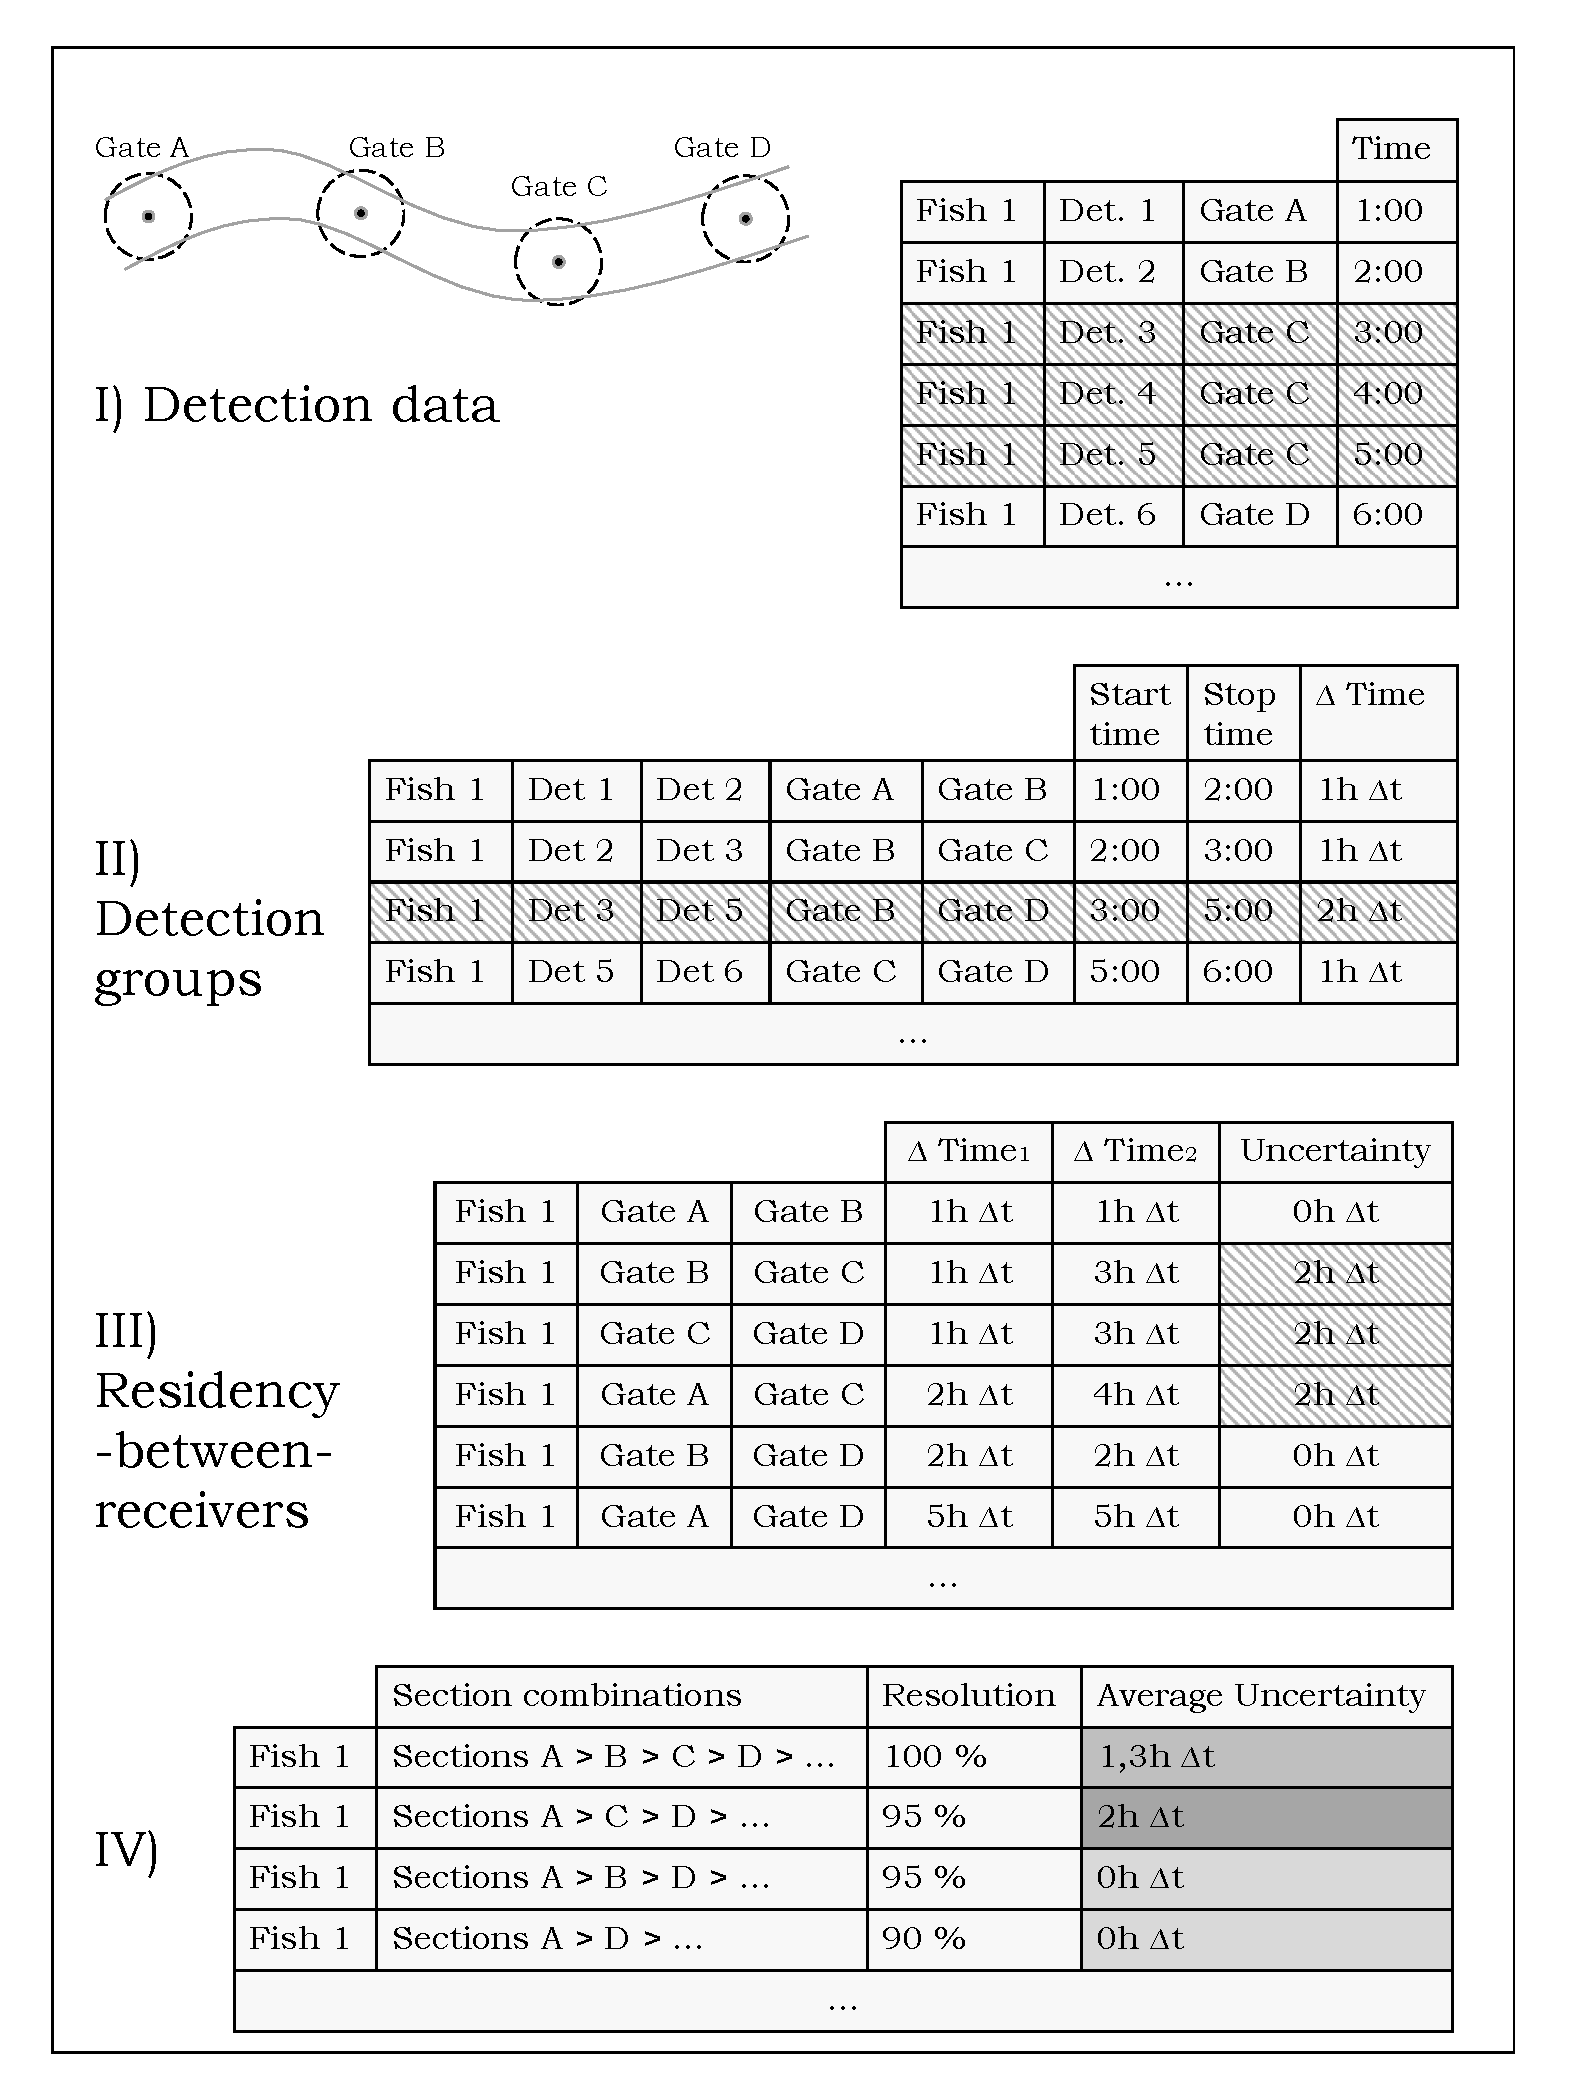
\includegraphics[scale=0.38]{Flow_chart.pdf}
  \caption{Data processing of detection data. I) The shaded detections were all tied up to one specific gate but it is unknown whether the tagged fish resided left or right of the gate during this period. This will introduce some epistemic uncertainty. II) Detections are transformed to detection groups. The shaded detections are combined in one detection group. III) Residencies-between-receivers are estimated from the detection groups. $\bigtriangleup$Time$_{1}$ and $\bigtriangleup$Time$_{2}$ represent the lower and upper bound of the residency-between-receivers intervals respectively. The epistemic uncertainty of the shaded detections is quantified. IV) Section combinations for different gate network resolutions are calculated. For a gate network resolution of 95 \% The section combination A,C,D has a higher average epistemic uncertainty than combination A,B,D. Hence, the latter is retained.}
  \label{fig:Flow_chart}
\end{figure}

\clearpage

\section{Tables}

\setcounter{table}{0} \renewcommand{\thetable}{C.\arabic{table}}
\setcounter{figure}{0} \renewcommand{\thefigure}{C.\arabic{figure}}

\begin{table}[h!]
\centering
\scriptsize
\caption{Detection probability of the entire network (ZS+WS), the Zeeschelde (ZS) section and the Westerschelde (WS) section for tagged eel. Because of the potentially large gaps between the receivers of the gates closer to the sea, assuming that fish were present between these gates may be erroneous. Therefore, we calculated the detection probability for two different scenarios. For scenario 1 we assumed that tagged fish reach the North Sea either way, even when they are not detected at any of the last three gates. For scenario 2 we assumed that tagged fish only reach the North Sea when they are detected at the last gate or at the network of the North Sea. \label{tab:det.prob.cases}}
\begin{tabular}{|l|l|l|l|} 
\hline
\multirow{2}{*}{Scenario} & \multicolumn{3}{l|}{Det. prob. (\% at section ...~ )}  \\ 
\cline{2-4}
                          & ZS+WS & ZS   & WS                                      \\ 
\hline
1                         & 92.3  & 95.8 & 46.4                                    \\ 
\hline
2                         & 95.5  & 97.0 & 62.5                                    \\
\hline
\end{tabular}
\end{table}

\begin{table}
\centering
\scriptsize
\caption{List of gates, with distance from Ghent (km), deployment date, number of included receivers, period of receiver inactivity and detection probability. Receiver inactivity represents the period during which one receiver of the gate was inactive. For example, four receivers of Gate ws2 were inactive during four different periods, which are given in the table.}
\label{gate list}
\begin{tabular}{|c|c|c|c|c|c|} 
\hline
\begin{tabular}[c]{@{}c@{}}gate\\name \end{tabular} & \begin{tabular}[c]{@{}c@{}}Distance\\(km) \end{tabular} & \begin{tabular}[c]{@{}c@{}}Deployment\\date \end{tabular} & \begin{tabular}[c]{@{}c@{}}number\\of receivers \end{tabular} & receiver inactivity          & \begin{tabular}[c]{@{}c@{}}Det. prob. (\%\\eel (flounder)\end{tabular}  \\ 
\hline
s1                                                  & 0.0                                                     & 31/03/2015                                                & 1                                                       &                         & 100.0                                                                   \\ 
\hline
s2                                                  & 6.6                                                     & 20/03/2016                                                & 1                                                       &                         & 100.0                                                                   \\ 
\hline
s3                                                  & 12.1                                                    & 20/03/2016                                                & 1                                                       &                         & 97.1                                                                    \\ 
\hline
s4                                                  & 16.8                                                    & 20/04/2015                                                & 1                                                       &                         & 97.4                                                                    \\ 
\hline
s5                                                  & 26.7                                                    & 31/03/2015                                                & 1                                                       &                         & 99.1                                                                    \\ 
\hline
s6                                                  & 30.6                                                    & 2/04/2015                                                 & 1                                                       &                         & 98.7                                                                    \\ 
\hline
s7                                                  & 33.0                                                    & 24/03/2016                                                & 1                                                       & 17/10/2017 - 24/11/2017 & 96.7                                                                    \\ 
\hline
s8                                                  & 39.3                                                    & 24/03/2016                                                & 1                                                       &                         & 81.6                                                                    \\ 
\hline
s9                                                  & 40.8                                                    & 20/04/2015                                                & 1                                                       &                         & 99.9                                                                    \\ 
\hline
s10                                                 & 44.1                                                    & 20/04/2015                                                & 1                                                       &                         & 99.3                                                                    \\ 
\hline
s11                                                 & 46.5                                                    & 27/04/2015                                                & 1                                                       &                         & 100.0                                                                   \\ 
\hline
s12                                                 & 49.0                                                    & 2/04/2015                                                 & 1                                                       &                         & 98.4                                                                    \\ 
\hline
s13                                                 & 53.8                                                    & 2/04/2015                                                 & 1                                                       &                         & 93.2                                                                    \\ 
\hline
s14                                                 & 55.6                                                    & 2/04/2015                                                 & 1                                                       &                         & 100.0                                                                   \\ 
\hline
s15                                                 & 63.3                                                    & 2/04/2015                                                 & 2                                                       &                         & 100.0 (87.5)                                                            \\ 
\hline
s16                                                 & 68.6                                                    & 2/04/2015                                                 & 2                                                       &                         & 100.0 (66.7)                                                            \\ 
\hline
s17                                                 & 75.8                                                    & 30/09/2015                                                & 3                                                       &                         & 100.0 (0)                                                               \\ 
\hline
s18                                                 & 88.2                                                    & 3/09/2015                                                 & 2                                                       &                         & 77.8 (50.0)                                                             \\ 
\hline
ws1                                                 & 112.8                                                   & 22/09/2015                                                & 6                                                       &                         & 91.3 (50.0)                                                             \\ 
\hline
ws2                                                 & 135.1                                                   & 1/07/2012                                                 & 21                                                      & 1/7/2012 - 29/12/2014   & 45.2 (33.3)                                                             \\ 
\cline{5-5}
                                                    &                                                         &                                                           &                                                         & 30/12/2014 - 22/2/2015  &                                                                         \\ 
\cline{5-5}
                                                    &                                                         &                                                           &                                                         & 15/10/2014 - 10/2/2015  &                                                                         \\ 
\cline{5-5}
                                                    &                                                         &                                                           &                                                         & 30/1/2014 - 11/2/2015   &                                                                         \\ 
\hline
ws3                                                 & 154.5                                                   & 22/05/2014                                                & 12                                                      & 15/1/2015 - 19/3/2015   & 29.2                                                                    \\ 
\cline{5-5}
                                                    &                                                         &                                                           &                                                         & 8/5/2015 - 9/9/2015     &                                                                         \\
\hline
\end{tabular}
\end{table}

\begin{table}
\centering
\scriptsize
\caption{List of tagged eels, with last station detected, detection probability, and tag power output (PO; L = low power output, H = high power output).}
\label{tag_list}
\begin{tabular}{|c|c|c|c|} 
\hline
Eel tag code            & Last station detected & Det. prob. (\%) & PO  \\ 
\hline
A69-1601-52623 & ws3                   & 100.0                & H   \\ 
\hline
A69-1601-52625 & ws3                   & 100.0                & H   \\ 
\hline
A69-1601-52635 & ws3                   & 100.0               & H   \\ 
\hline
A69-1601-52645 & ws3                   & 100.0                & H   \\ 
\hline
A69-1601-52649 & ws3                   & 100.0                & H   \\ 
\hline
A69-1601-52632 & ws3                   & 97.0                 & H   \\ 
\hline
A69-1601-52662 & ws3                   & 95.7                 & H   \\ 
\hline
A69-1602-30330 & ws2                   & 95.5                 & H   \\ 
\hline
A69-1602-30333 & ws3                   & 95.2                 & H   \\ 
\hline
A69-1601-52642 & ws2                   & 95.0                 & H   \\ 
\hline
A69-1601-52622 & ws3                   & 94.7                 & H   \\ 
\hline
A69-1601-52629 & ws3                   & 94.7                 & H   \\ 
\hline
A69-1601-52633 & ws3                   & 94.7                 & H   \\ 
\hline
A69-1601-52636 & ws3                   & 94.7                 & H   \\ 
\hline
A69-1601-52647 & ws3                   & 94.7                 & H   \\ 
\hline
A69-1601-52654 & ws3                   & 94.7                 & H   \\ 
\hline
A69-1602-30346 & ws3                   & 94.7                 & H   \\ 
\hline
A69-1601-57472 & ws2                   & 93.8                 & L   \\ 
\hline
A69-1602-30352 & ws1                   & 92.9                 & H   \\ 
\hline
A69-1601-52644 & ws3                   & 91.2                 & H   \\ 
\hline
A69-1601-52639 & ws1                   & 90.9                 & H   \\ 
\hline
A69-1602-30332 & ws1                   & 90.9                 & H   \\ 
\hline
A69-1602-30331 & ws3                   & 90.9                 & H   \\ 
\hline
A69-1602-30337 & ws2                   & 90.5                 & H   \\ 
\hline
A69-1601-52653 & ws1                   & 90.0                 & H   \\ 
\hline
A69-1602-30343 & ws1                   & 90.0                & H   \\ 
\hline
A69-1602-30345 & ws1                   & 90.0                & H   \\ 
\hline
A69-1602-30355 & ws1                   & 90.0                & H   \\ 
\hline
A69-1602-30344 & ws3                   & 90.0                 & H   \\ 
\hline
A69-1601-52641 & ws2                   & 89.5                 & H   \\ 
\hline
A69-1601-52648 & ws2                   & 89.5                 & H   \\ 
\hline
A69-1601-52651 & ws2                   & 89.5                 & H   \\ 
\hline
A69-1602-30356 & ws1                   & 88.9                 & H   \\ 
\hline
A69-1601-52664 & ws3                   & 88.9                 & H   \\ 
\hline
A69-1602-30350 & ws3                   & 88.9                & H   \\ 
\hline
A69-1601-52638 & s18                   & 85.0                 & H   \\ 
\hline
A69-1601-57475 & ws3                   & 85.0                 & L   \\ 
\hline
A69-1601-57470 & ws1                   & 80.0                 & L   \\
\hline
\end{tabular}
\end{table}

\begin{table}
\centering
\scriptsize
\caption{Output of the fixed effects of the linear mixed effects model with log-transformed epistemic uncertainty as response, gate network resolution and removed station as fixed effect and eel as random effect. The values, standard errors (SE), degrees of freedom (DF), t-values and p-values are given. The p-values of the post-hoc tests of the factor removed station were corrected using the Bonferroni approach. Only comparisons resulting in significant p-values are given. For the original combinations of sections bordered by gates no gates were omitted.}
\label{lmer model stations removed}
\resizebox{\columnwidth-235pt}{!}{%
\begin{tabular}{|l|l|l|l|l|l|}
\hline
Coefficient & SE   & DF    & t-value & p-value & Effect       \\ \hline
0.11        & 0.00 & 12742 & 406.02  & 0.00    & resolution   \\ \hline
-11.50      & 0.14 & 12742 & -84.32  & 0.00    & intercept    \\ \hline
0.40        & 0.04 & 12742 & 10.48   & 0.00    & original-ws2 \\ \hline
0.39        & 0.04 & 12742 & 10.15   & 0.00    & original-ws1 \\ \hline
0.32        & 0.04 & 12742 & 8.35    & 0.00    & original-s4  \\ \hline
0.31        & 0.04 & 12742 & 8.23    & 0.00    & original-s12 \\ \hline
0.31        & 0.04 & 12742 & 8.20    & 0.00    & original-s2  \\ \hline
0.31        & 0.04 & 12742 & 8.03    & 0.00    & originals-18 \\ \hline
0.30        & 0.04 & 12742 & 7.95    & 0.00    & original-s17 \\ \hline
0.26        & 0.04 & 12742 & 6.86    & 0.00    & original-s15 \\ \hline
0.26        & 0.04 & 12742 & 6.81    & 0.00    & original-s9  \\ \hline
0.25        & 0.04 & 12742 & 6.64    & 0.00    & original-s8  \\ \hline
0.25        & 0.04 & 12742 & 6.49    & 0.00    & s10-ws2      \\ \hline
0.25        & 0.04 & 12742 & 6.34    & 0.00    & s11-ws2      \\ \hline
0.24        & 0.04 & 12742 & 6.29    & 0.00    & original-s16 \\ \hline
0.24        & 0.04 & 12742 & 6.28    & 0.00    & original-s7  \\ \hline
0.24        & 0.04 & 12742 & 6.16    & 0.00    & s10-ws1      \\ \hline
0.23        & 0.04 & 12742 & 6.00    & 0.00    & s11-ws1      \\ \hline
0.22        & 0.04 & 12742 & 5.63    & 0.00    & s14-ws2      \\ \hline
0.22        & 0.04 & 12742 & 5.58    & 0.00    & s6-ws2       \\ \hline
0.21        & 0.04 & 12742 & 5.56    & 0.00    & original-s3  \\ \hline
0.21        & 0.04 & 12742 & 5.52    & 0.00    & original-s5  \\ \hline
0.21        & 0.04 & 12742 & 5.41    & 0.00    & s13-ws2      \\ \hline
0.20        & 0.04 & 12742 & 5.30    & 0.00    & s14-ws1      \\ \hline
0.20        & 0.04 & 12742 & 5.25    & 0.00    & s6-ws1       \\ \hline
0.20        & 0.04 & 12742 & 5.07    & 0.00    & s13-ws1      \\ \hline
0.19        & 0.04 & 12742 & 5.02    & 0.00    & original-s13 \\ \hline
0.19        & 0.04 & 12742 & 4.90    & 0.00    & s5-ws2       \\ \hline
0.19        & 0.04 & 12742 & 4.86    & 0.00    & s3-ws2       \\ \hline
0.18        & 0.04 & 12742 & 4.83    & 0.00    & original-s6  \\ \hline
0.18        & 0.04 & 12742 & 4.79    & 0.00    & original-s14 \\ \hline
0.18        & 0.04 & 12742 & 4.56    & 0.00    & s5-ws1       \\ \hline
0.18        & 0.04 & 12742 & 4.53    & 0.00    & s3-ws1       \\ \hline
0.17        & 0.04 & 12742 & 4.38    & 0.00    & s10-s4       \\ \hline
0.16        & 0.04 & 12742 & 4.25    & 0.00    & s10-s12      \\ \hline
0.16        & 0.04 & 12742 & 4.23    & 0.00    & s10-s2       \\ \hline
0.16        & 0.04 & 12742 & 4.22    & 0.00    & s11-s4       \\ \hline
0.16        & 0.04 & 12742 & 4.15    & 0.01    & s7-ws2       \\ \hline
0.16        & 0.04 & 12742 & 4.14    & 0.01    & s16-ws2      \\ \hline
0.16        & 0.04 & 12742 & 4.09    & 0.01    & s11-s12      \\ \hline
0.16        & 0.04 & 12742 & 4.08    & 0.01    & s11-s2       \\ \hline
0.16        & 0.04 & 12742 & 4.06    & 0.01    & s10-s18      \\ \hline
0.15        & 0.04 & 12742 & 4.06    & 0.01    & original-s11 \\ \hline
0.15        & 0.04 & 12742 & 3.99    & 0.01    & s10-s17      \\ \hline
0.15        & 0.04 & 12742 & 3.91    & 0.02    & s11-s18      \\ \hline
0.15        & 0.04 & 12742 & 3.90    & 0.02    & original-s10 \\ \hline
0.15        & 0.04 & 12742 & 3.83    & 0.02    & s11-s17      \\ \hline
0.15        & 0.04 & 12742 & 3.84    & 0.02    & s8-ws2       \\ \hline
0.15        & 0.04 & 12742 & 3.81    & 0.03    & s7-ws1       \\ \hline
0.15        & 0.04 & 12742 & 3.81    & 0.03    & s16-ws1      \\ \hline
\end{tabular}
}
\end{table}

\FloatBarrier

\section{Figures}

\setcounter{table}{0} \renewcommand{\thetable}{D.\arabic{table}}
\setcounter{figure}{0} \renewcommand{\thefigure}{D.\arabic{figure}}

\begin{figure}[h!]
  \centering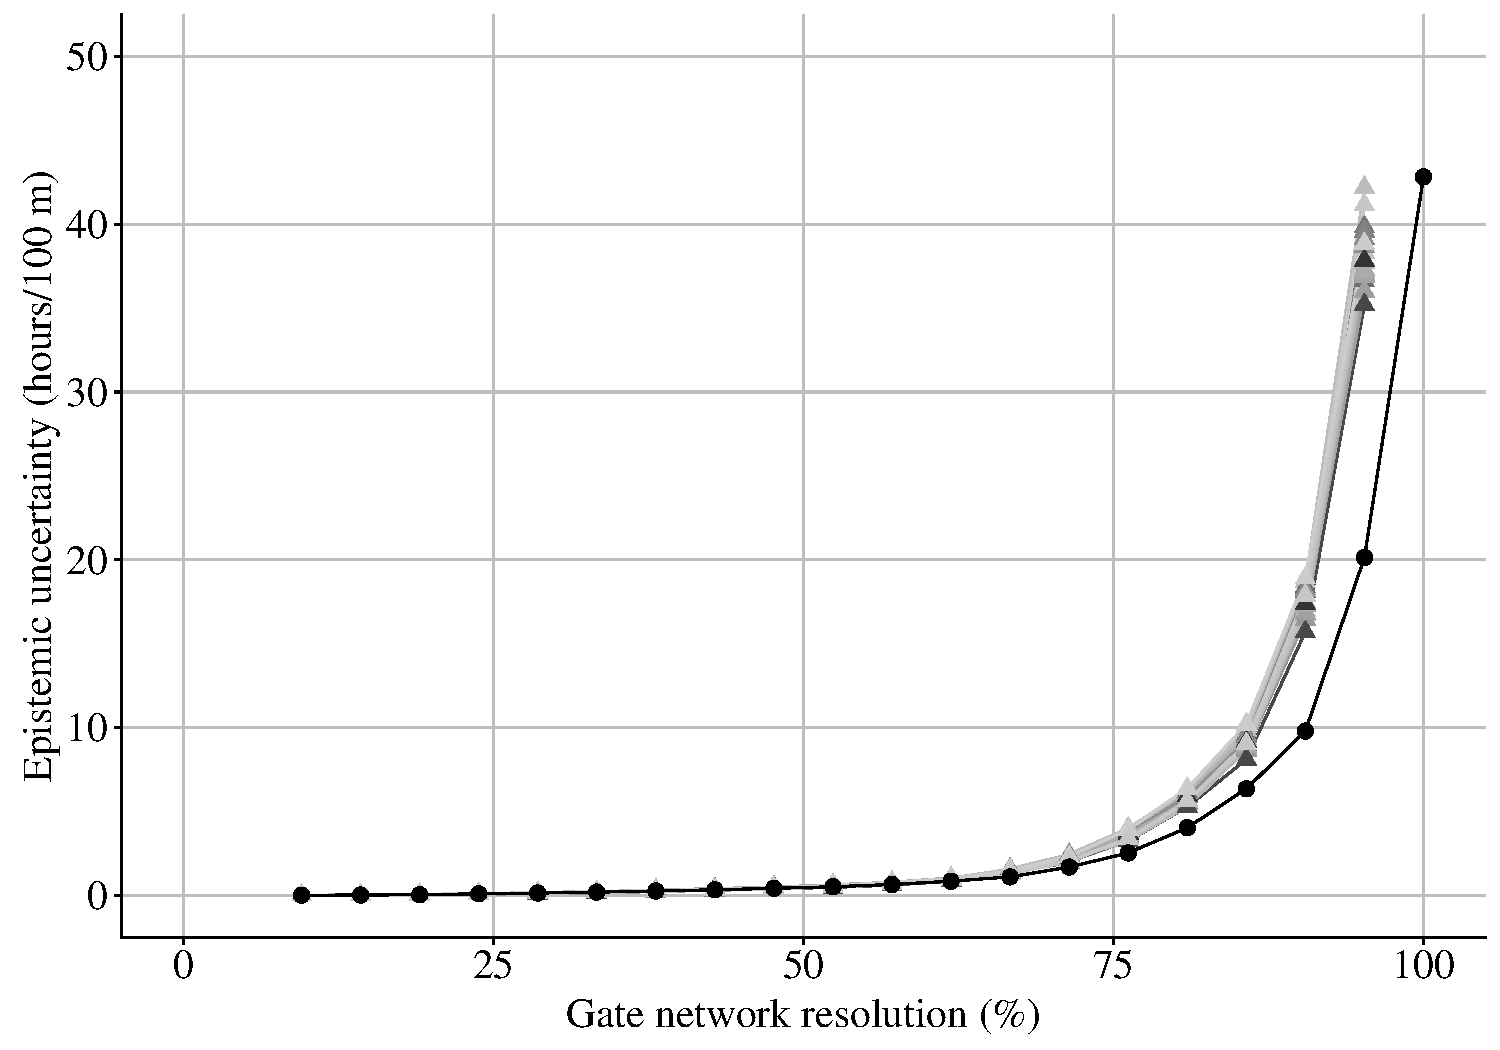
\includegraphics[scale=0.45]{Pareto_stations_removed_duration.pdf}
  \caption{Effect of omitting specific gates on trade-off between epistemic uncertainty (vertical axis) and gate network resolution (horizontal axis). The average trade-off of all 38 eels was calculated. Each curve with triangle dots represents different section combination trade-offs with different gates being omitted. The black curve with the circle dots represents the original trade-off without any gates being omitted.}
  \label{fig:Pareto_stations_removed}
\end{figure}

\begin{figure}[h!]
  \centering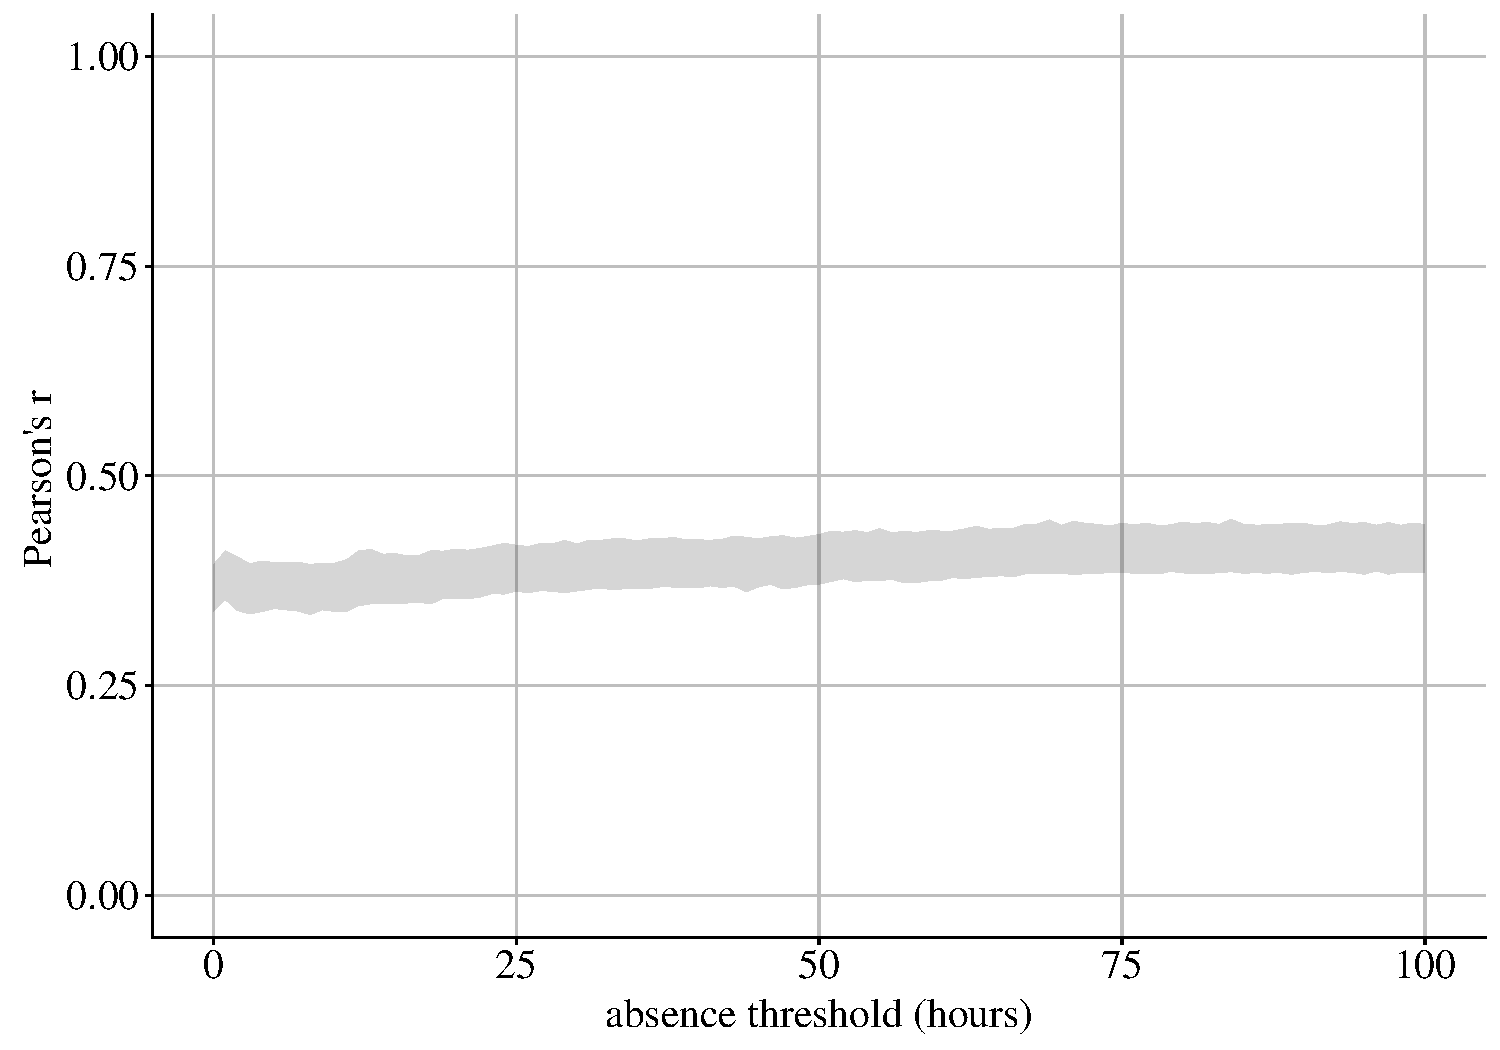
\includegraphics[scale=0.45]{correlation_activity_and_gate_period.pdf}
  \caption{Pearson's correlation coefficient ($r$) of residencies-between-receivers and residencies-at-receivers for different absence threshold values. Monte Carlo simulations (10$^{6}$) were used to determine the band of possible $r$ values.}
  \label{fig:correlation}
\end{figure}

\begin{figure}[h!]
  \centering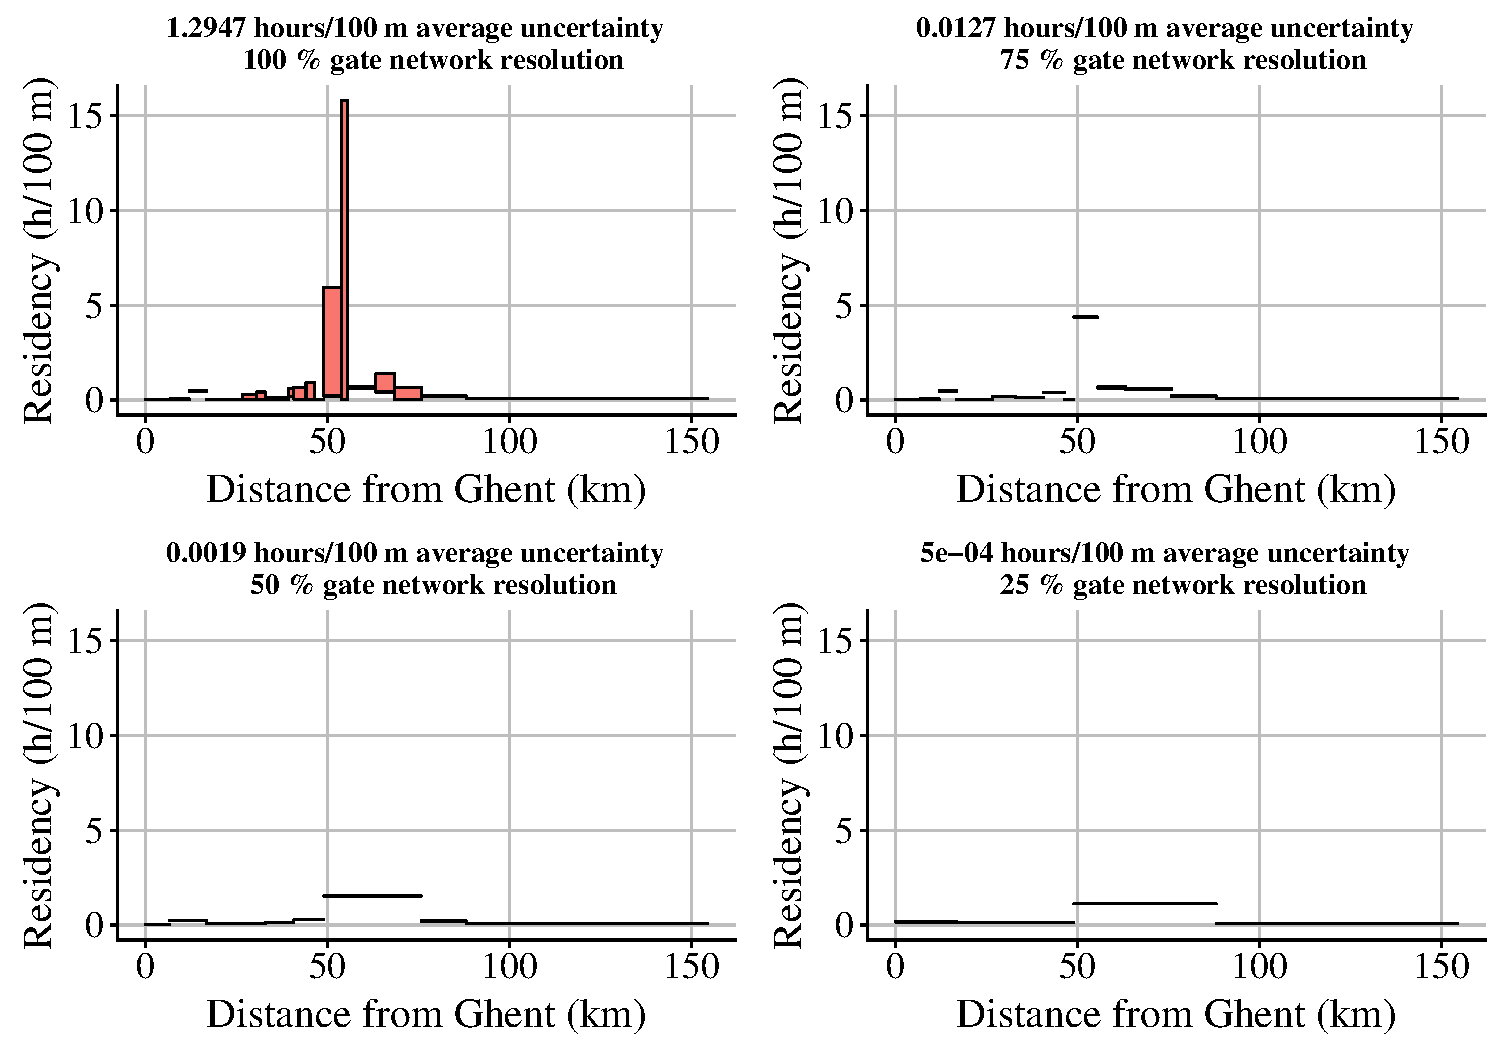
\includegraphics[scale=0.45]{Resistance_model2_jb_eel2.pdf}
  \caption{Residency-between-receivers (hours/100m) in function of distance from Ghent (km). Combinations of sections bordered by gates for eel "A69-1601-52623" with different levels of gate network resolution and different levels of average epistemic uncertainty are depicted. The range between the minimum and maximum value of the residencies-between-receivers, i.e. the epistemic uncertainty, is represented by the red boxes.}
  \label{fig:Resistance_model2}
\end{figure}

\begin{figure}[h!]
  \centering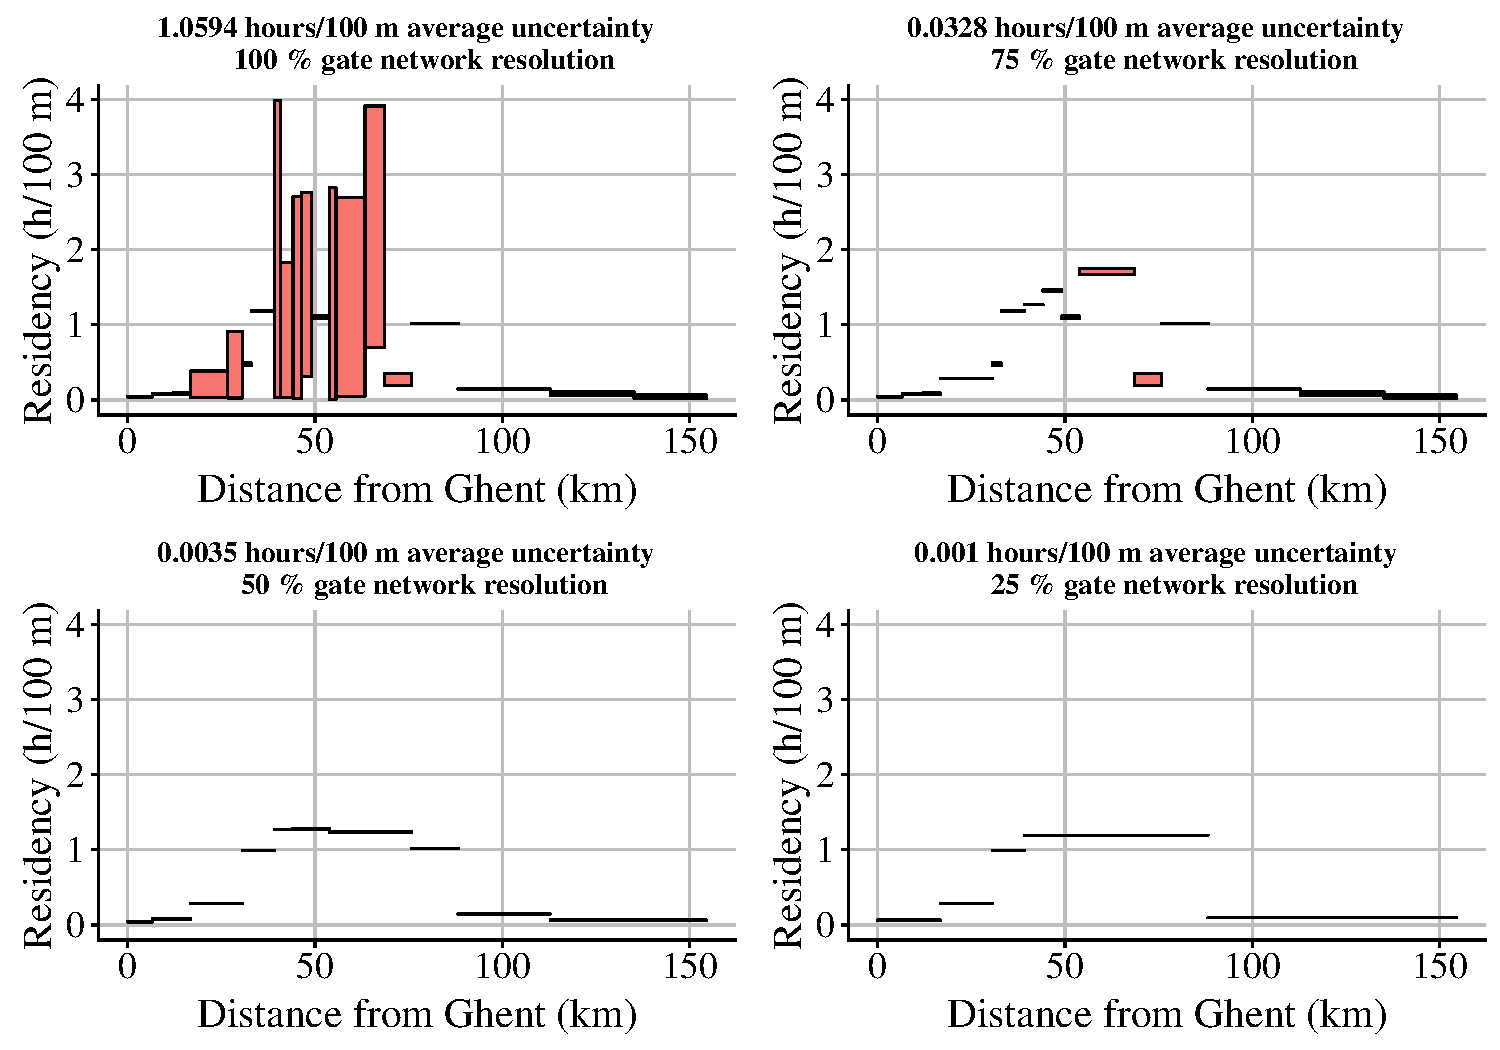
\includegraphics[scale=0.45]{Resistance_model2_jb_eel3.pdf}
  \caption{Residency-between-receivers (hours/100m) in function of distance from Ghent (km). Combinations of sections bordered by gates for eel "A69-1601-52625" with different levels of gate network resolution and different levels of average epistemic uncertainty are depicted. The range between the minimum and maximum value of the residencies-between-receivers, i.e. the epistemic uncertainty, is represented by the red boxes.}
  \label{fig:Resistance_model3}
\end{figure}

\FloatBarrier

\section{Population assessment}
\label{Fig}

\setcounter{table}{0} \renewcommand{\thetable}{E.\arabic{table}}
\setcounter{figure}{0} \renewcommand{\thefigure}{E.\arabic{figure}}

Different tagged eels have different optimal combinations of sections bordered by gates for a specific gate network resolution. For different resolutions, different sections are combined to obtain an optimal reduction in epistemic uncertainty. It is possible to assign each section between gates a midpoint value of the corresponding residency-between-receivers interval, but it should be noted that with decreasing gate network resolution the results are smoothed and spatial information gets lost. A high gate network resolution on the other hand, has the advantage of providing a unique estimate for many different sections, but generally the unaccounted uncertainty of these sections will be high. In Fig. \ref{fig:overall_uncertainty} can be seen that at a gate network resolution of 100 \%, the high level of epistemic uncertainty obscures any potential trend, while at a gate network resolution of 25 \% the extensive loss of spatial information smoothes any potential trend away. It seems that for this case, a gate network resolution of 50 \% allows to detect a simple trend in the duration that eels spend between the different sections.  

\begin{figure}[h!]
  \centering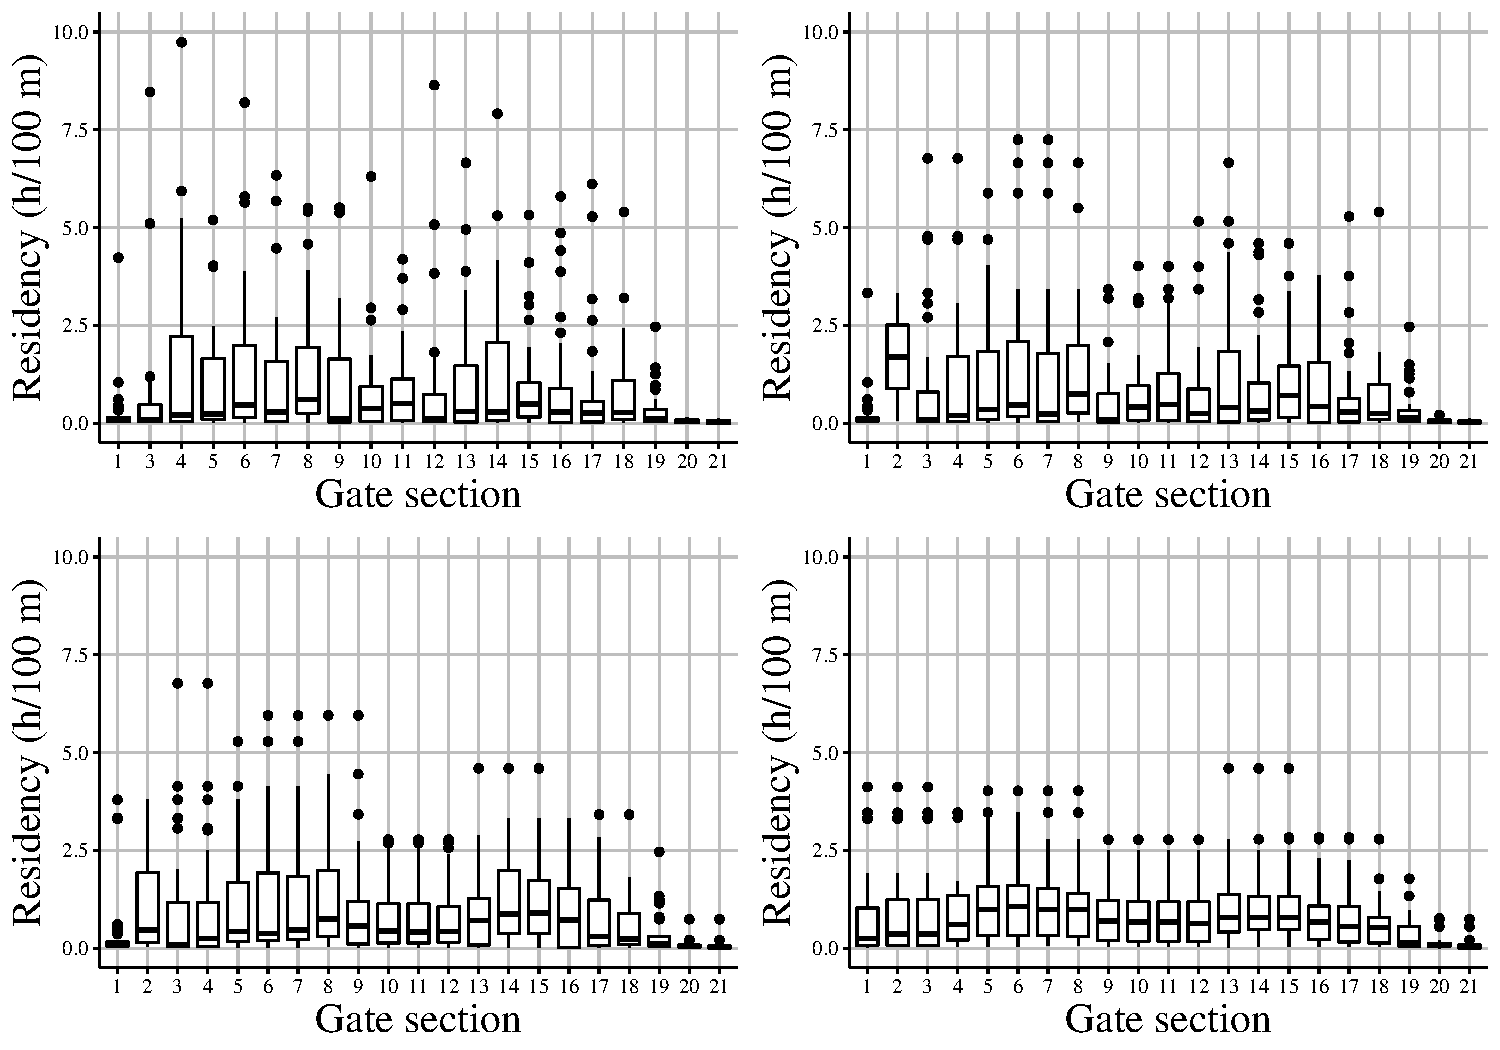
\includegraphics[scale=0.45]{overall_uncertainty.pdf}
  \caption{Boxplots of midpoint values of all residency-between-receivers intervals of all tagged eels.}
  \label{fig:overall_uncertainty}
\end{figure}